\subsection{Current State}
\label{current_state}
% Current state:
  % Cloud computing
    % High latencies
    % large data centres
    % AWS/Azure/hadoop

Cloud computing enables computing resources to be available to users remotely, so that users do not need to actively manage the compute hardware.
This is often motivated by economies of scale, in that the greater quantity of computing resources you are managing, the cheaper it becomes per unit.
Cloud computing also makes it easier for a user to scale the resources they are using, since this is simply done by increasing or decreasing a regular payment, instead of buying or selling hardware. This can be particularly attractive to small businesses or individuals.

Cloud computing has been slowly but steadily rising in popularity since the release of the first cloud computing platform: Amazon's Elastic Compute Cloud (EC2) \cite{ec2}.
This was released in 2006 \cite{announce_ec2}, has since grown significantly, and inspired many competitors, such as Microsoft Azure \cite{azure} and Google Cloud Platform \cite{google_cloud}.

Since cloud computing intends to serve the computing requirements of large numbers of users, there are naturally hardware requirements that need to be filled by the cloud computing provider.
This is normally done in the form of data centres, which are large buildings filled with servers and the appropriate infrastructure to make those servers accessible remotely. For an example of the scale that a large cloud computing provider requires, AWS has 64 ``availability zones'' around the world where ``each AZ can be multiple data centers (typically 3), and at full scale can be hundreds of thousands of servers.'' \cite{aws_infrastructure_blog}.

When a cloud computing platform hosts a customer's data, that data is stored on one of the servers owned by the platform in one of their data centres. A good platform will replicate the data in case of hardware failure, but generally the data would only be served from a single data centre, unless the customer pays for the data to be hosted in more locations.
Whenever data is requested over a network, there is a delay involved in retrieving that data, much of which arises from the geographical distance that the data has to travel. A user located in Australia will have a longer delay after requested data hosted in an American data centre, than someone requesting the same data who lives in America.
This issue, partially caused by the rise in cloud computing and, as a result, data centres, is a key motivation for this project.

\begin{figure}[ht]
  \centering
  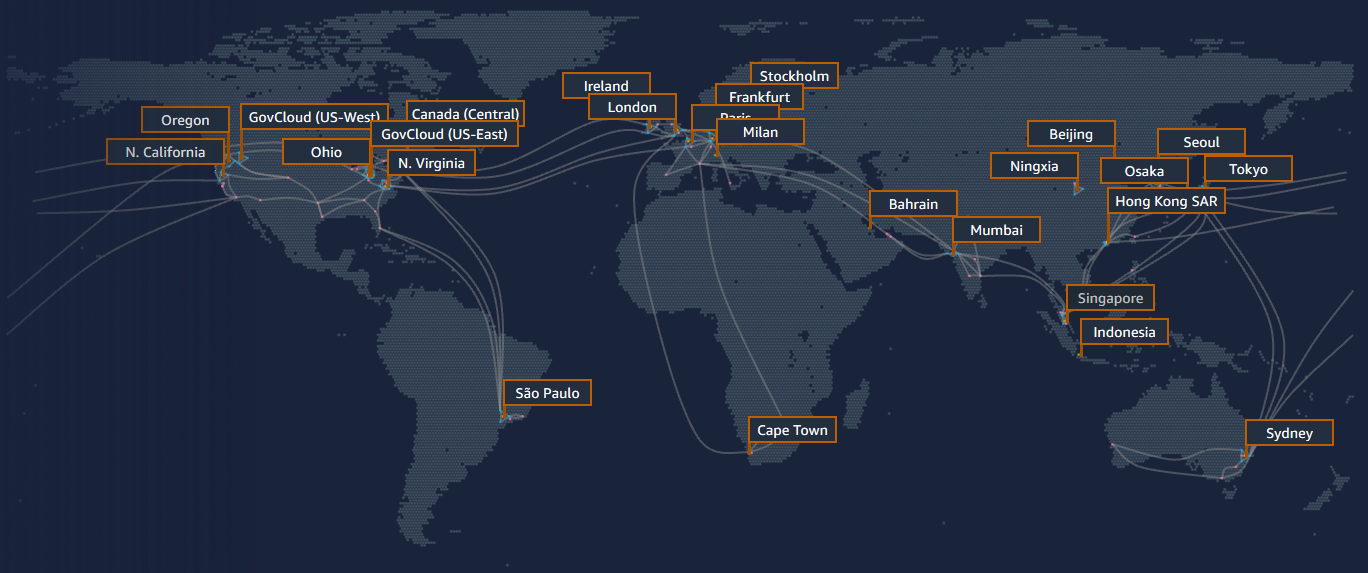
\includegraphics[width=\textwidth]{assets/aws_infrastructure.png}
  \caption{Regions of AWS}
  \label{aws_regions}
\end{figure}

\subsection{Existing Solutions}
\label{existing_solutions}
% Existing solutions and issues
  % Mainframes
    % inflexible
    % high maintenance
    % single point of failure
    % very expensive
    % more
  % "edge" / "gateway" nodes
    % essentially just small data centres
    % similar downsides
  % NetFPGA
    % doesn't solve problem
  % SDN
    % doesn't solve problem

  % Other drawbacks
    % security
    % scalability
    % Flexibility
    % performance

Some methods have been designed to reduce the time taken for data to travel between a user and a cloud server.
One of these methods is `edge' or `gateway' nodes.
Edge nodes are comparable to data centres, with the key difference being that they are significantly smaller. They exist to hold content closer to users, so that not all content needs to be retrieved all the way from the data centre. Edge nodes are often used to host tools intended to manage the data centre, such as tools for customers to manage the data they have stored on a cloud computing platform.

While edge nodes do improve the service, they suffer from many of the same drawbacks as data centres. In addition, the more edge nodes a cloud computing platform creates, the more difficult it is for the provider to manage their hardware, as it becomes spread out over a larger geographical area.

Before cloud computing became widely popular, it was necessary for users to host their own files. For those with large data requirements, it was not uncommon to use mainframe computers. These are large, high performance server computers, generally built and sold as a unit. Those using a mainframe would process all of their data on site. This would allow for data to be processed with an extremely low latency.

However, mainframe computers became unpopular for all the reasons cloud computing grew in popularity. Mainframe computers require significant on-site management. They require a high up-front cost, constant running costs in terms of power and cooling, are physically large and loud, and can be difficult to scale.

\subsection{Project Solution}
\label{project_solution}
% Why this, and why this is different?
  % Don't divert data from current path.
    % It's heading to data centre, so use that path.
  % choose appropriate device
    % ASIC vs FPGA vs CPU


The approach this project has taken in solving the above problem has been comprised of two parts:
\begin{enumerate}
  \item By not altering the path of the data, any data which would need to travel the full path would not be slowed.
  \item Choosing an appropriate device to perform the computation.
\end{enumerate}

\subsubsection{Maintaining Data Path}

This approach led to the idea of FPGA-based smart network switches. These switches could replace standard network switches, and would be able to perform small amounts of computation on data as it passed through these switches. If data was able to be fully processed by the switch, it would then be returned to the device, without ever needing to be sent to the data centre. If the switch was unable to complete the computation within a set amount of time, it would release the data in its partially processed state along its original path, where it would then meet either further FPGA-based smart network switches, or its destination server. If it met further FPGA-based smart network switches prior to reaching its destination server, these could perform additional processing on the data, leading to a higher chance of completing the computation for a set of data.

\subsubsection{Choosing a Device for Computation}

The devices considered for use as computation devices in these smart switches were FPGAs, ASICs, and CPUS. Each of these have different advantages and disadvantages over one another. Three of the main areas of comparison were speed, flexibility, and cost.

The fastest of these three devices are ASICs. ASICs compute the algorithm they are designed for in hardware, and they are capable of doing so very efficiently.
Since FPGAs are designed to be more flexible than ASICs, ASICs can achieve greater speeds than FPGAs for the same algorithm.
CPUs are significantly slower than both ASICs and FPGAs, since they perform computation in software, rather than in hardware. In addition, unlike ASICs and FPGAs, CPUs are not standalone devices. They require additional hardware in order to function, including RAM, a motherboard, possibly storage, and often additional cooling. This would mean that any data the CPU would need to process would have to flow through an Ethernet interface which, for a high bandwidth Ethernet connection may need to be an NIC connected through a PCIe interface, then through the motherboard, then the RAM, then the CPU cache, and finally through the CPU registers, before it could be processed. While there will also be more than one stage to process data using an FPGA or ASIC, this is far more complex with a CPU.

While ASICs are the best for speed, they are the worst for flexibility. ASICs are by definition application-specific, meaning that they are designed to perform one algorithm, and that is the only algorithm which they are capable of performing. In order to achieve the flexibility required for this project, different ASICs would need to be designed for each algorithm required by a user, and the smart switches would then have to be physically swapped out to change the algorithm. This would also be inordinately expensive, and is unlikely to be manufacturable.
FPGAs are significantly more flexible than ASICs. They can be programmed using either HDLs such as \textit{Verilog} or \textit{VHDL}, or some high-level languages such as \textit{C} or \textit{C++} using sophisticated synthesis tools. In addition, FPGAs support advanced techniques such as `Partial Reconfiguration', which allow blocks of an FPGA to be declared as `reconfigurable', and these blocks can then be swapped out during runtime, without stopping the execution of the remainder of the program running on the FPGA.
CPUs are the most flexible of the devices, again due to their ability to run programs in software. This allows them to run programs using most modern programming languages, including 2019's ``most loved languages'', \textit{Rust} and \textit{Python} \cite{stack_overflow_dev_survey_2019}.
However, as mentioned above, CPUs are not standalone devices. Their requirement for additional hardware restricts their flexibility, since it increases their physical size.

Cost is the most difficult means of comparing devices, since there are many different parameters to take into account. The cheapest devices available are consumer CPUs, which can cost less than £100 for a low end desktop CPU \cite{scan_celeron_g4900} \cite{intel_celeron_g4900}, or over £2000 for a high end server CPU \cite{scan_xeon_gold_6132} \cite{intel_xeon_gold_6132}.
However, these are consumer prices, and assume the purchase of only one product.
% However, even these prices cannot be considered entirely accurate, since they assume the purchase of only one device.
It is more difficult to find accurate prices for FPGAs and ASICs, but a comparison of the two can be seen in figure \ref{fpga_asic_cost_tradeoff}. ASICs have a much higher initial cost, but a lower cost per unit compared to FPGAs.
However, FPGAs are a very active research area, and their cost per unit is slowly decreasing, causing the break even point shown in figure \ref{fpga_asic_cost_tradeoff} to slowly shift to the right, making FPGAs more cost-effective than ASICs.

FPGAs were chosen as the optimal computation device for this project. ASICs are insufficiently flexible, and even with their advantages in speed, they are subsequently not suitable for this task. CPUs, while more flexible than FPGAs, are significantly slower, and would be impractical to combine with a network switch. FPGAs are fast, flexible, and sufficiently small devices, and are the most suitable tool available.

\begin{figure}[ht!]
  \centering
  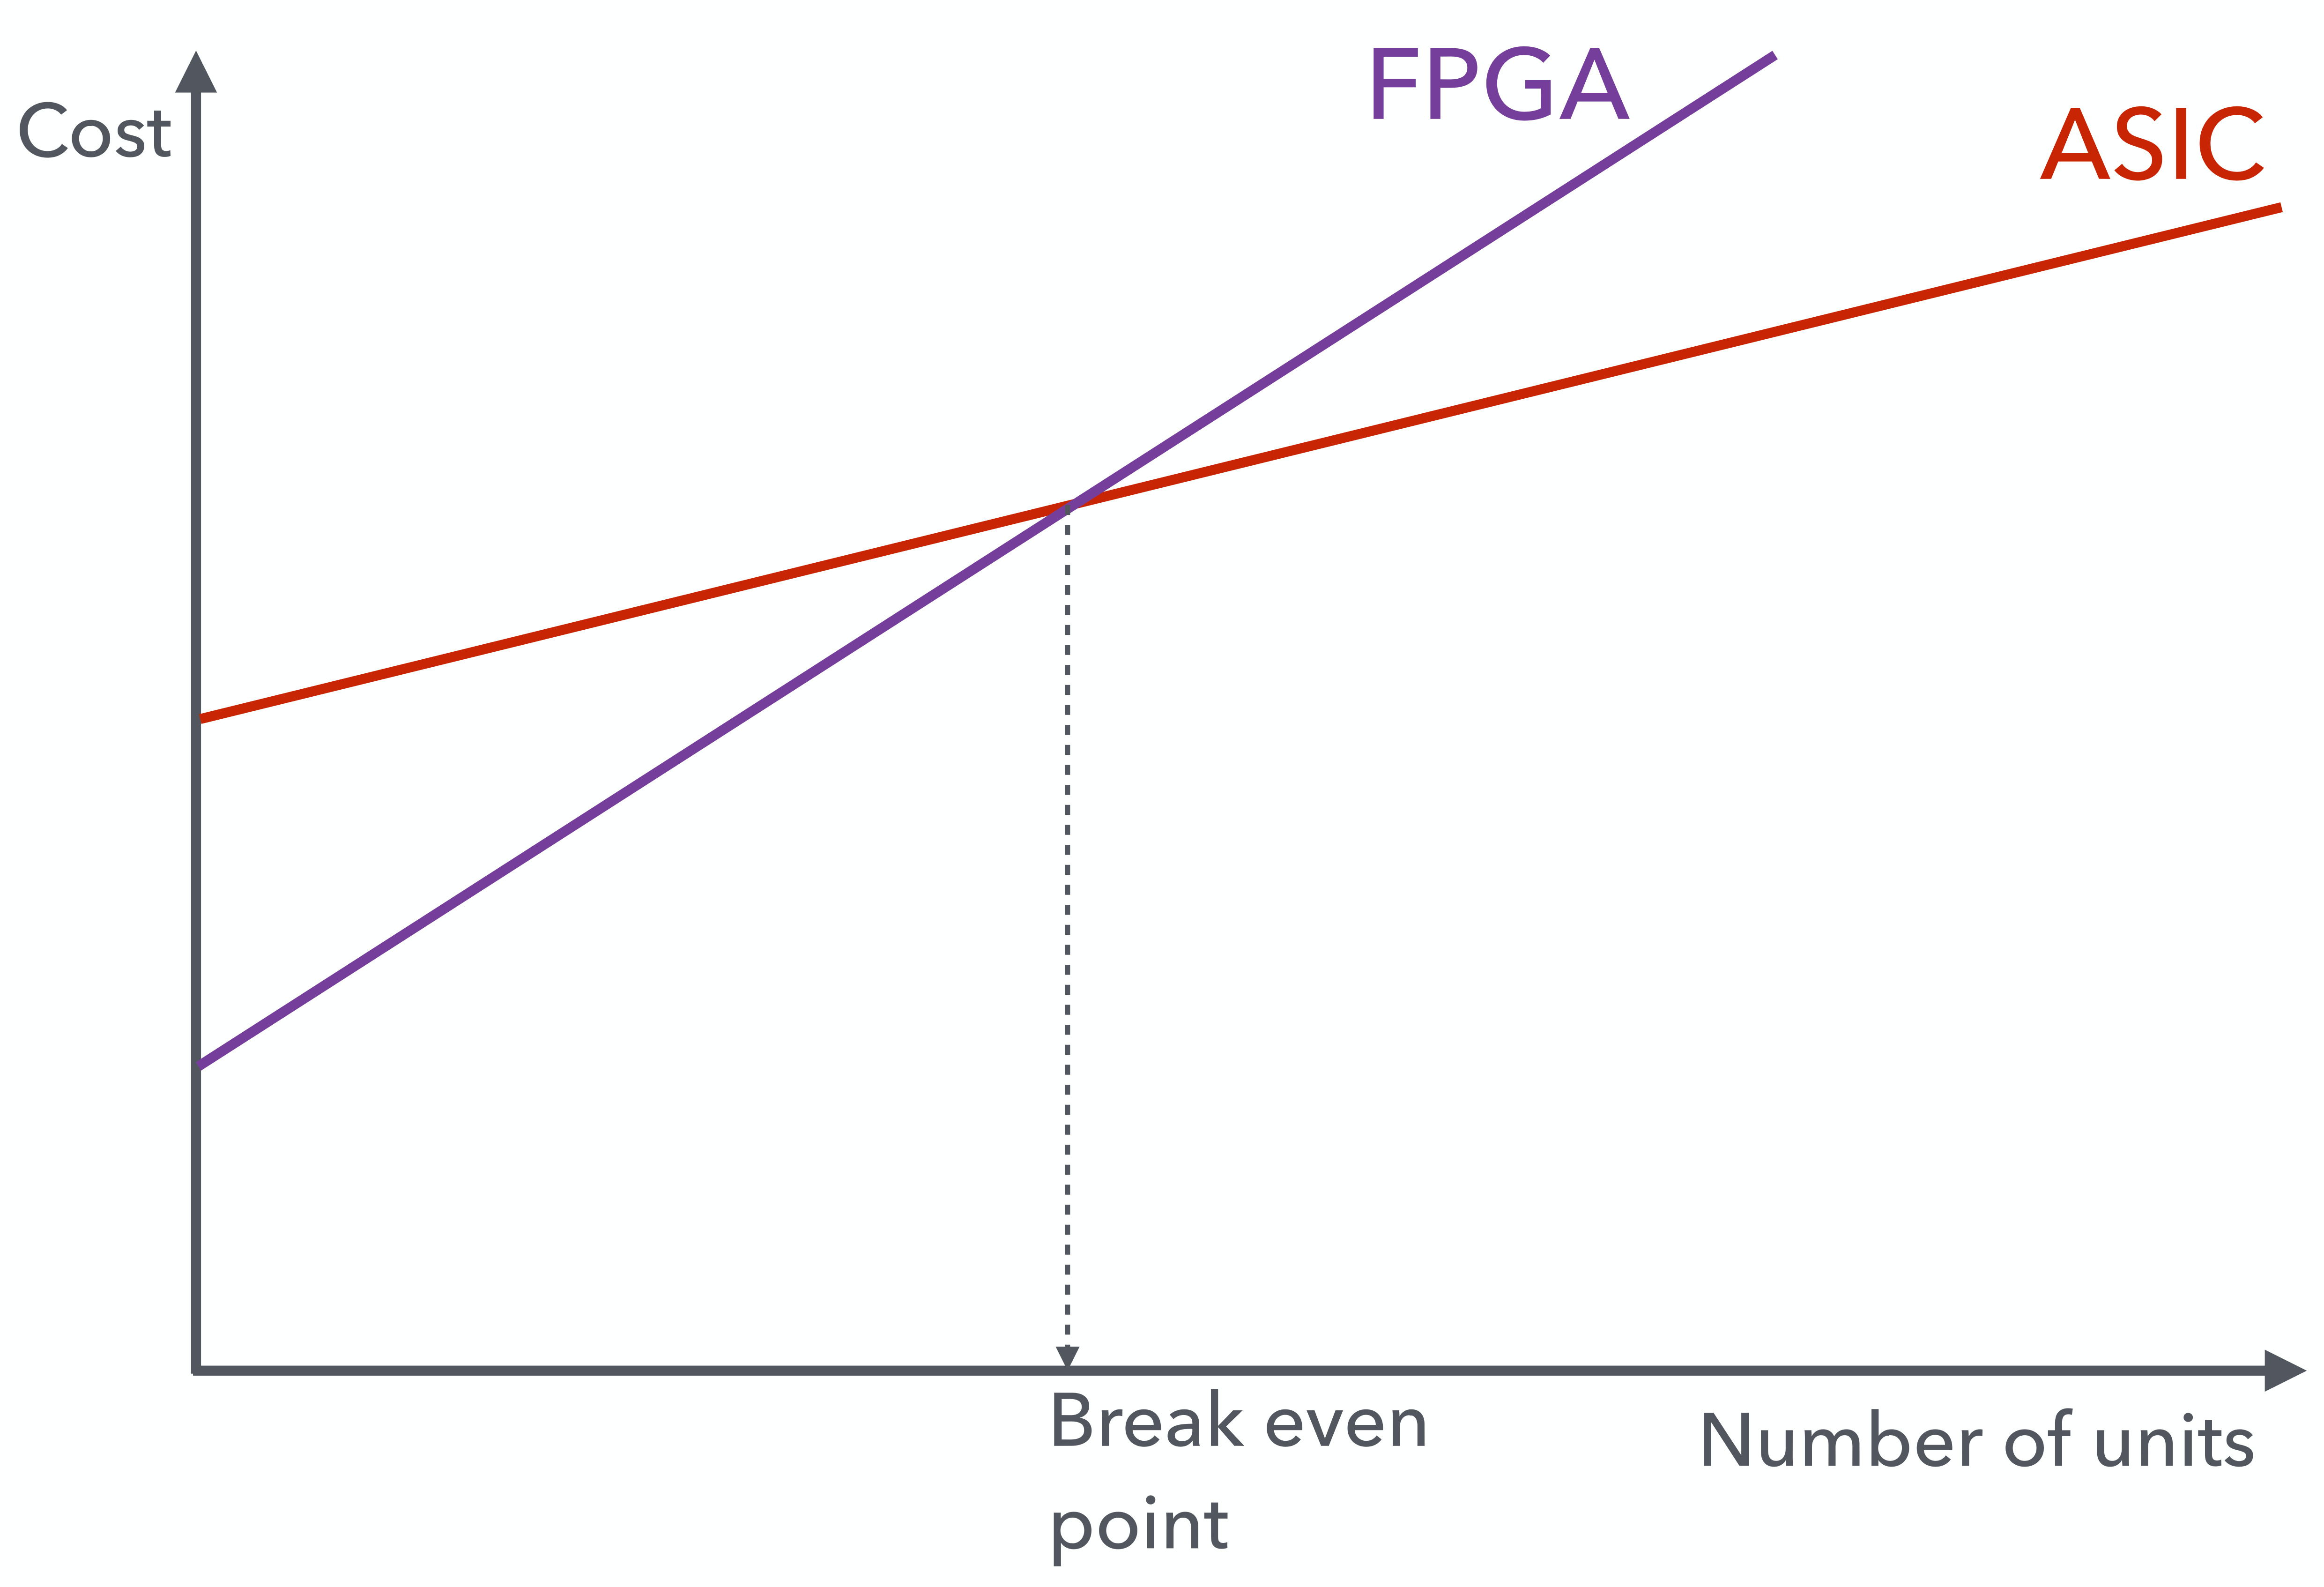
\includegraphics[width=\textwidth]{assets/fpga_asic_cost_tradeoff.png}
  \caption{Comparison of FPGA and ASIC cost \cite{es3b2}}
  \label{fpga_asic_cost_tradeoff}
\end{figure}


% Why FPGAs?
  % Custom compute architectures - very low latency
  % why not CPU? (bring data in through NIC -> mobo -> mem -> cache -> reg -> CPU -> back out)
    % FPGA just in and out
  % Partial reconfiguration
